\documentclass[12pt]{article}
\usepackage[russian]{babel}
\usepackage[utf8x]{inputenc}
\usepackage{amssymb}
\usepackage{amsmath}
\usepackage{graphicx}
\usepackage[margin=.7in]{geometry}
\usepackage[colorinlistoftodos]{todonotes}
\usepackage{listings}
\usepackage[section]{placeins}
\usepackage[T1]{fontenc}
\begin{document}

\title{Оценка параметров систем массового обслуживания}
\author{Андрей Валиков}
\date{}
\maketitle

\section{Цель работы}
Оценить следующие характеристики коммутаторов: вероятность потерь вызова, производительность, среднее число соединений. Лабораторная работа выполнена на языке Python 3.6 с использованием библиотек Matplolib и SciPy и представляет собой модели, позволяющие исследовать характеристики однозвенных коммутаторов при различных параметрах.

\section{Общая модель коммутатора}
Коммутатор в данной работе представляет собой модель, имеющую $M$ входов и $N$ выходов.

\begin{figure}[htp]
\centering
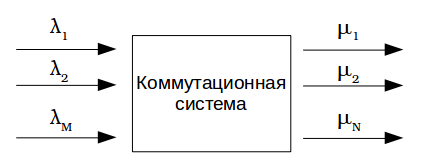
\includegraphics[scale=1.00]{comm_model.png}
\end{figure}


\section{Параметры системы}\label{sec:systemParams}

\begin{tabular}{l l}
    $M$ & входы коммутатора \\
    $N$ & выходы коммутатора \\
    $\lambda$ & поступление нагрузки на одном входе \\
    $\mu$ & уход нагрузки с одного выхода \\
    $P$ & вероятность потерь вызовов \\
    $G$ & производительность \\
    $E$ & среднее число соединений \\
\end{tabular} \\
    $\rho = \frac{\lambda}{\mu}$ -- отношение поступления нагрузки к её уходу 

																																																							

\section{Вероятность блокировки для трёх распредлений}\label{sec:prob}


\subsection{Распределение Энгсета}\label{subsec:engset}

 \[
     p = \frac{\rho ^ N \binom{M}{N}}
     {\sum_{n=0}^{N} \rho ^ n \binom{M}{n}}
 \]

\subsection{Распределение Эрланга}\label{subsec:erlang}

\[
     p = \frac{(M \rho) ^ N}
     {N!\sum_{n=0}^{N + 1} \frac{(M \rho) ^ n}{n!}}
\]

\subsection{Биноминальное распределение}\label{subsec:binom}
Пусть $\alpha = \frac{\lambda}{\mu + \lambda}$

\[
     p = \binom{M}{N} \alpha ^ N (1 - \alpha) ^ {M - N}
\]

\section{Код программы}

\begin{lstlisting}

import math
import matplotlib.pyplot as plt
import numpy as np
import scipy.misc as scipy_misc

fact = math.factorial

l_range = np.arange(.01, 1, .05)

mu = .9

M, N = 20, 10

comb = scipy_misc.comb(M, N)


P1_k, G1_k, E1_k = [], [], []
P2_k, G2_k, E2_k = [], [], []
P3_k, G3_k, E3_k = [], [], []


def p_engset(lam):
    _sum = sum((scipy_misc.comb(M, n) * ((lam / mu) ** n) for n in range(N + 1)))
    return comb * (((lam / mu) ** N) / _sum)


def p_erlang(lam):
    _sum = sum(((M * lam / mu) ** n) / fact(n) for n in range(N + 2))
    return (M * lam / mu) ** N / (fact(N) * _sum)


def p_binom(lam):
    alpha = lam / (mu + lam)
    return comb * (alpha ** N) * (1 - alpha) ** (M - N)


def perf(lam, p):
    """performance"""
    return lam * M * (1 - p)


def cons(lam, p):
    """connections"""
    return perf(lam, p) / mu


def common_plot(**kwargs):
    plt.title((kwargs['title'] + ' M={}, N={}, mu={}').format(M, N, mu))
    plt.plot(l_range, kwargs['engset'], label='Engset')
    plt.plot(l_range, kwargs['erlang'], label='Erlang')
    plt.plot(l_range, kwargs['binom'], label='Binom')
    plt.legend()
    plt.show()


for l in l_range:
    P1_k.append(p_engset(l))
    G1_k.append(perf(l, P1_k[-1]))
    E1_k.append(cons(l, P1_k[-1]))

    P2_k.append(p_erlang(l))
    G2_k.append(perf(l, P2_k[-1]))
    E2_k.append(cons(l, P2_k[-1]))

    P3_k.append(p_binom(l))
    G3_k.append(perf(l, P3_k[-1]))
    E3_k.append(cons(l, P3_k[-1]))

common_plot(title='Loss probabitlty', engset=P1_k, erlang=P2_k, binom=P3_k)
common_plot(title='Performance', engset=G1_k, erlang=G2_k, binom=G3_k)
common_plot(title='Average connexitions number',   engset=E1_k, erlang=E2_k, binom=E3_k)
\end{lstlisting}

\section{Результат}

\subsection{$M = N$}

\begin{figure}[!htb]
\centering
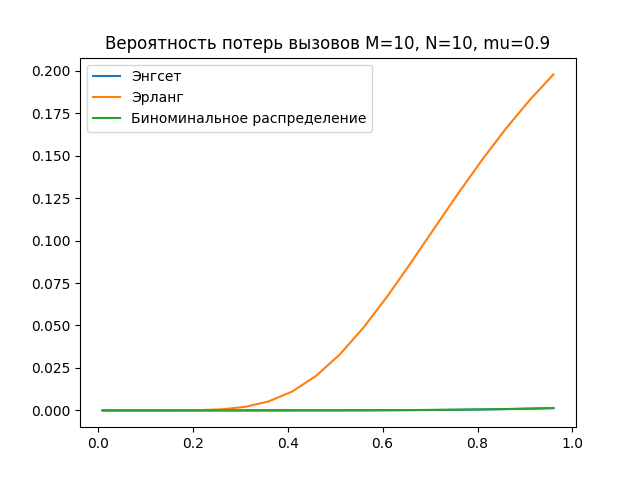
\includegraphics[scale=1.00]{loss_prob_M10_N10_mu09.png}
\caption{}
\label{}
\end{figure}

\begin{figure}[!htb]
\centering
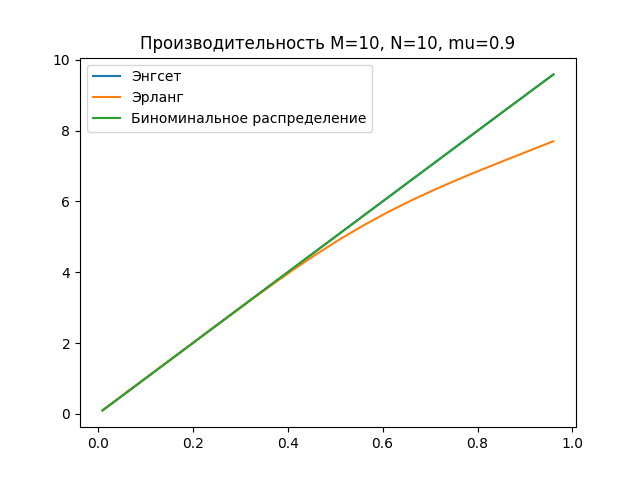
\includegraphics[scale=1.00]{perf_M10_N10_mu09.png}
\caption{}
\label{}
\end{figure}

\begin{figure}[!htb]
\centering
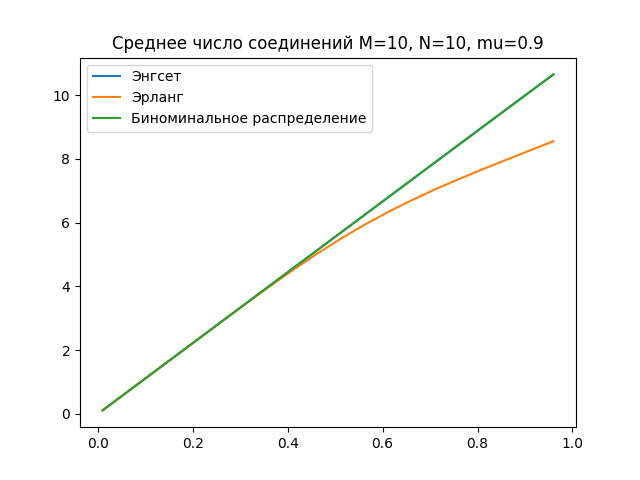
\includegraphics[scale=1.00]{aver_conn_M10_N10_mu09.png}
\caption{}
\label{}
\end{figure}

\subsection{$M ≫ N$}
\begin{figure}[!htb]
\centering
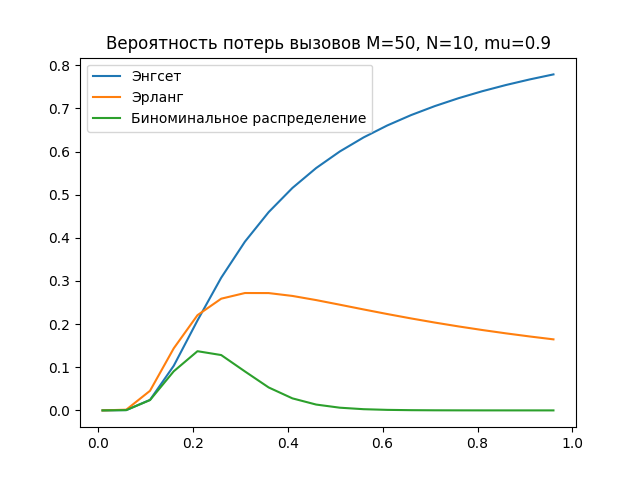
\includegraphics[scale=1.00]{loss_prob_M50_N10_mu09.png}
\caption{}
\label{}
\end{figure}

\begin{figure}[!htb]
\centering
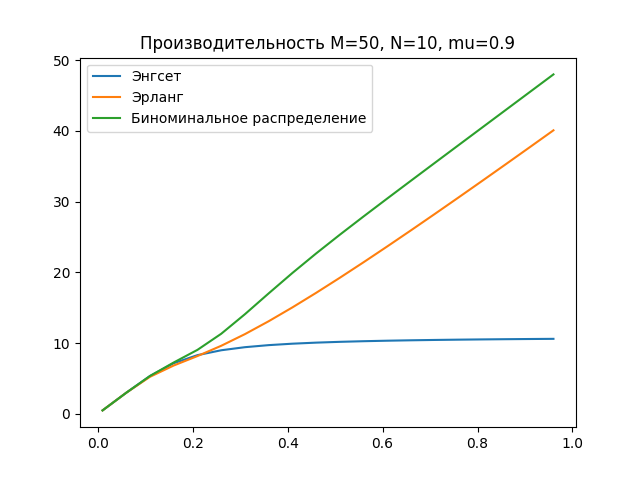
\includegraphics[scale=1.00]{perf_M50_N10_mu09.png}
\caption{}
\label{}
\end{figure}

\begin{figure}[!htb]
\centering
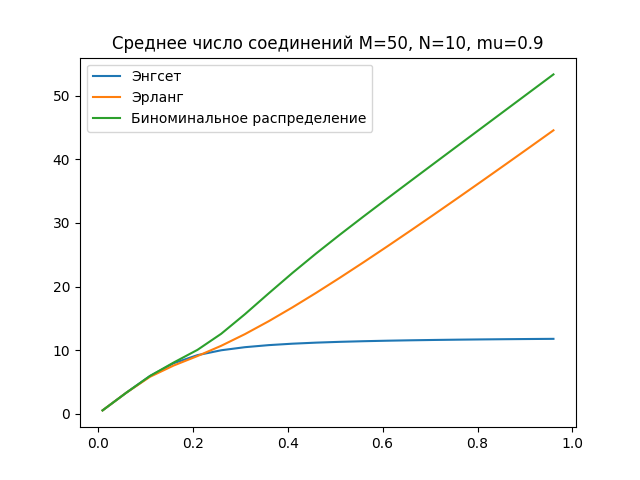
\includegraphics[scale=1.00]{aver_conn_M50_N10_mu09.png}
\caption{}
\label{}
\end{figure}

\section{Вывод}
При исследовании зависимости параметров коммутационной системы от интенсивности поступления нагрузки были получены следующие выводы:
\begin{itemize}
	\item При $M = N$:
	\begin{itemize}
		\item Наименьшая вероятность потерь вызовов с вероятностью поступления вызовов по распределению Эрланга или Биномиальному распределению
		\item Чем выше коэффициент интенсивности ухода потока нагрузки, тем лучше результат.
	\end{itemize}
	\item При $ M ≫ N$
		\begin{itemize}
			\item Наибольшая производительность системы
			\item Наиболее эффективный результат дает распределение Энгсета и Биномиальное распределение, $\mu$ при этом не имеет существенного влияния.
			\item Среднее число соединений в  системе также имеет наибольшее значение при наименьшем значении $\mu$, с подчинением закону распределения Энгсета и Биномиальному
		\end{itemize}
\end{itemize}

Параметры коммутатора во многом зависят от:
\begin{itemize}
	\item Закона распределения вероятностей поступающих заявок в систему
	\item $\lambda$
	\item $\mu$
	\item $\rho = \frac{\lambda}{\mu}$
	\item нормированной интенсивности поступления нагрузки
\end{itemize}
Для каждого конкретного случая необходимо учитывать все эти характеристики в совокупности для получения требуемых параметров системы.




\end{document}